\clearpage

\section{Компилятор графа вычислений}

Общая схема работы компилятора представлена на рис.~\ref{fig:compiler_scheme}. 
На вход ему поступает граф вычислений. Затем последний преобразуется в код на языке
диалекта высокого уровня. Этот код подвергается различным оптимизациям и
преобразованиям, после чего транслируется (<<понижается>>) в код на языке
диалекта низкого уровня. После очередной итерации преобразований низкоуровневый
диалект преобразуется в LLVM IR и передается в JIT-компилятор для генерации
машинного кода и исполнения. Полученный исполняемый модуль содержит вызовы к
библиотеке среды исполнения, которая отвечает за взаимодействие с физическими
устройствами и управление памятью.

\begin{figure}[h]
  \centering
  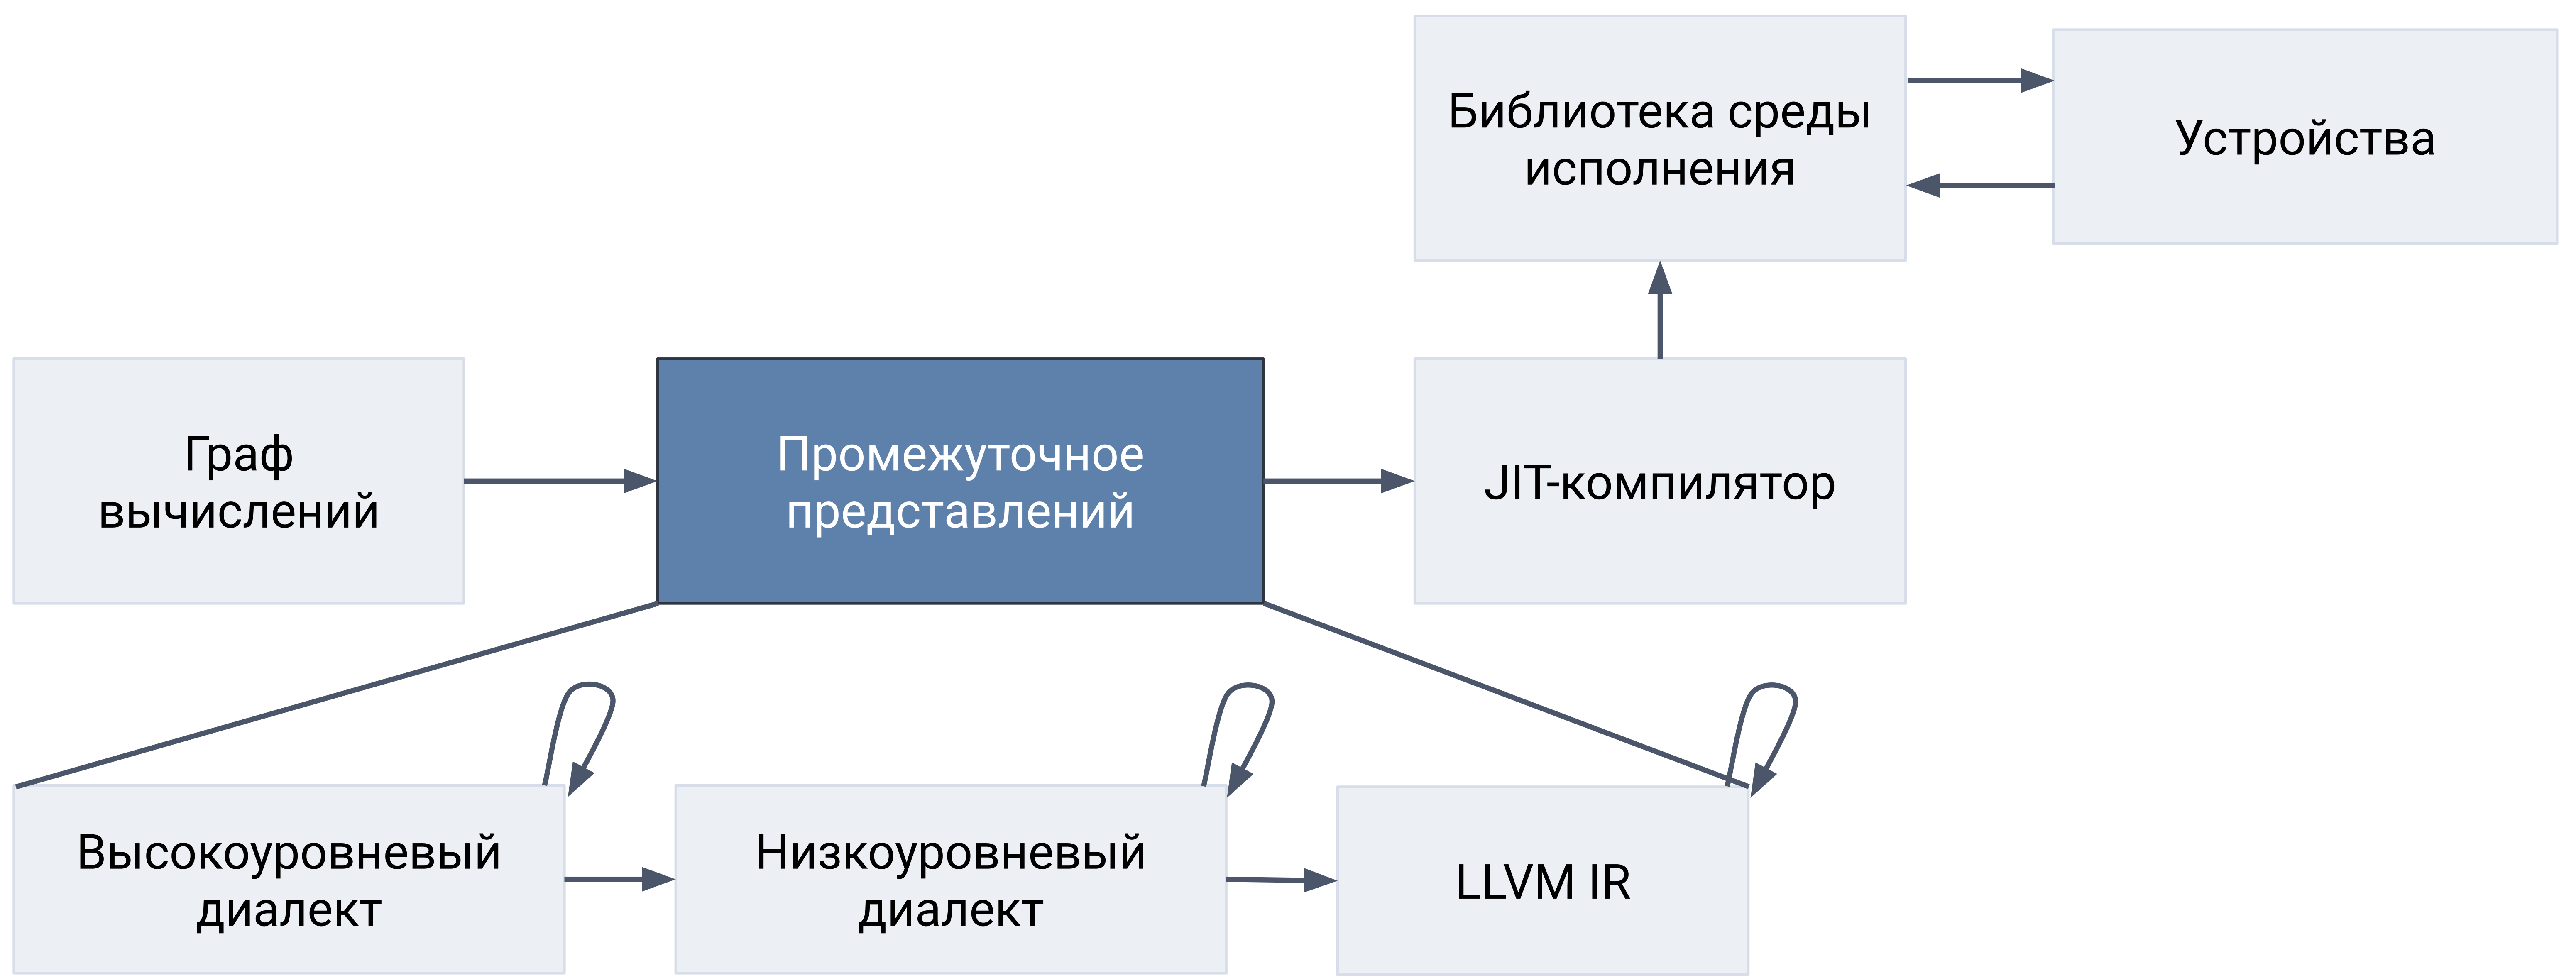
\includegraphics[width=\textwidth]{compiler_scheme}
  \caption{Схема работы компилятора графа вычислений}
  \label{fig:compiler_scheme}
\end{figure}
\subsection{Граф вычислений}

Рассмотрим пример простейшей функции:
\[
  f(x, y) = x + y.
\]
В простейшем случае можно представить эту функцию с помощью графа вычислений,
изображенного на рис.~\ref{fig:simple_add}. В то же время, существует множество
нюансов, о которых необходимо позаботиться, при вычислении данной функции.
Однозначно определить операцию сложения можно лишь для объектов (скаляров,
векторов, матриц, тензоров) одинаковых размеров и одинаковых типов данных.
Кроме того, необходимо позаботиться о выделении нужного объема памяти для
выполнения операции. Таким образом, граф должен включать в себя инофрмацию не
только о математических операциях, но и информацию о природе входных данных. 

\begin{figure}[h]
  \begin{subfigure}{.3\textwidth}
    \centering
    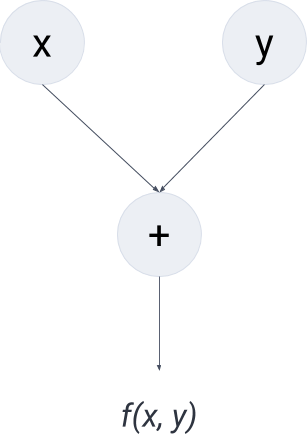
\includegraphics[width=0.8\linewidth]{simple_add}
    \caption{В простейшем случае}
    \label{fig:simple_add}
  \end{subfigure}
  \begin{subfigure}{.7\textwidth}
    \centering
    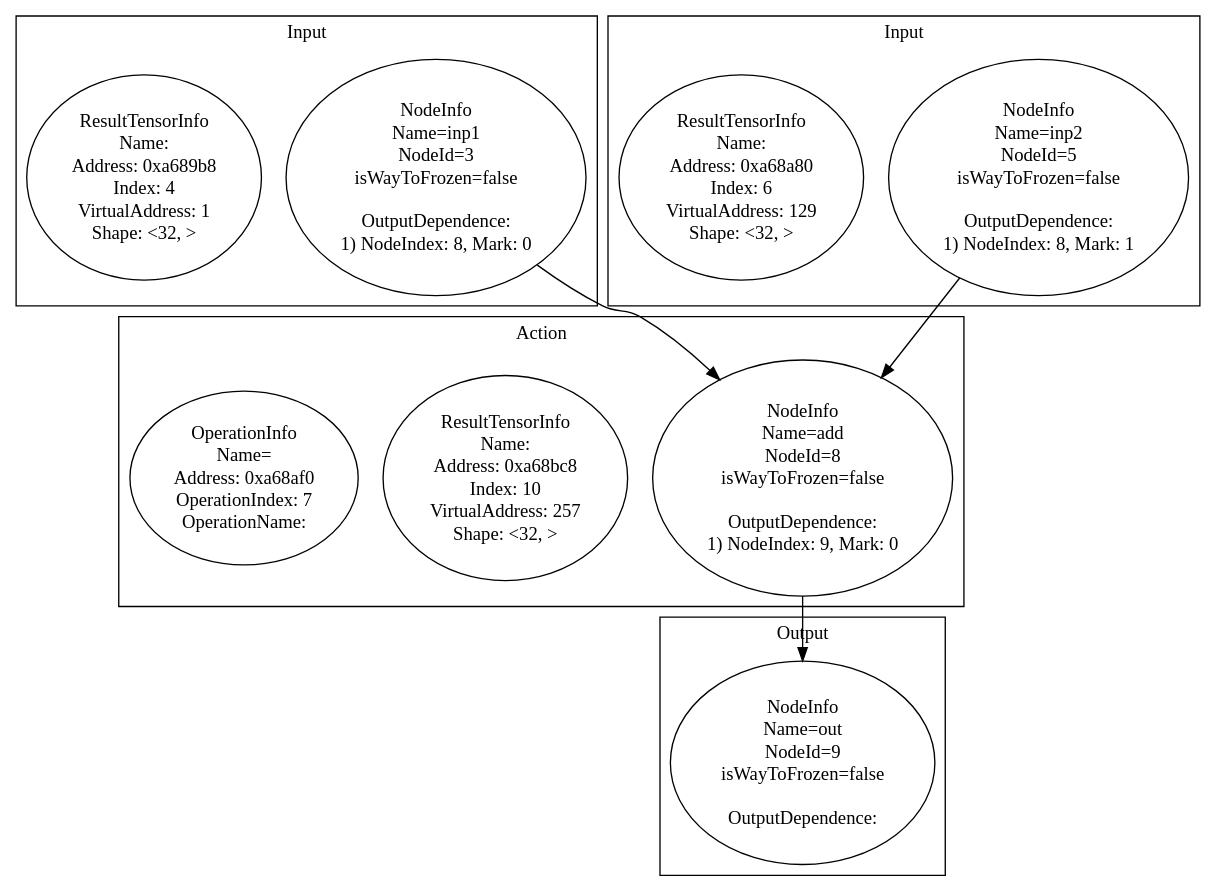
\includegraphics[width=\linewidth]{advanced_add}
    \caption{С учетом дополнительной информации}
    \label{fig:advanced_add}
  \end{subfigure}
  \caption{Пример графа вычислений для функции $f(x, y) = x + y$}
  \label{fig:add}
\end{figure}


Именно это показано на рис.~\ref{fig:advanced_add}. Такой граф содержит
информацию о типе вершины (входная, выходная, вычисления), размерность и тип
данных тензора, виртуальный адрес тензора и т.д. Этой инофрмации достаточно
для генерации исплняемого кода.

Чтобы выполнить преобразование, граф вычислений сперва разбивается на 
кластеры\footnote{Более подробно структура графа и алгоритм разбиения на кластеры
рассматриваются в работе \cite{graph}} таким образом, что вершины каждого нового кластера
зависят только от результатов вычислений вершин в предыдущих кластерах. Таоке
разбиение дает ряд преимуществ. Во-первых, вершины в пределах одного кластера
независимы, а значит их можно вычислять одновременно. Во-вторых, при обработке
кластеров можно так же добиться параллелизма. После того, как кластер $n$
закончил работу и передал следующему кластеру, он может вернуться к работе,
обрабатывая очередную порцию данных. В-третьих, упрощается преобразование графа
в код. Данная трансформация выполняется путем последовательного обхода кластеров
и генерации кода для принадлежащих ему вершин.

\subsection{Высокоуровневый диалект}
Задача высокоуровневого диалекта -- представить граф вычислений в доступном для
компилятора виде, сохранив при этом смысловую информацию о вычислениях.

Для моделирования данного диалекта будет использоваться описанная ранее
технология MLIR. С ее помощью будет сконструирован язык, похожий по свойствам
на язык LLVM IR, а так же разработаны инструментальные средства обработки
полученного промежуточного представления.

Основными компонентами программы на языке диалекта высокого уровня являются
вершины и графы. По своим свойствам они напоминают функции. Вершины могут 
принимать и возвращать значения. Графы же больше походят на функцию main и 
имеют строго определенную сигнатуру: не принимают и не возвращают значений.
Из тела <<функции>> графа происходят вызовы функций, вычисляющих вершины.
Кроме того, в графе содержатся специальные операции -- барьерные синхронизации.
Достигая такой операции, программа приостанавливает работу до завершения
начатых ранее вычислений. Вершины же описывают действия, которые необходимо
совершить для получения корректного результата. К ним относятся выделение памяти,
загрузка данных в память, математические операции, совершаемые над тензорами.

Помимо привычных типов данных, таких как целое число или число с плавающей
точкой, вводится специальный тип данных <<тензор>>. Тензор характеризуется
своей размерностью и типом данных элемента тензора. Размерность тензора может
быть не определена в момент построения промежуточного представления, но должна
быть выведена в ходе последующих преобразований.

\begin{lstlisting}[language=athgraph,caption=Различные варианты тензоров]
%0 = "ath_graph.create_tensor"() {virtual_address = 1 : index} : () -> tensor<2x2xf32> // Матрица 2x2
%1 = "ath_graph.create_tensor"() {virtual_address = 5 : index} : () -> tensor<?xf32> // Вектор неизвестной длины
%2 = "ath_graph.create_tensor"() {virtual_address = 9 : index} : () -> tensor<*xf32> // Тензор неизвестного ранга
\end{lstlisting}

Пример кода, полученного в результате компиляции графа для функции 
$f(x, y) = x + y$, приведен в листинге~\ref{lst:ath_graph_add} Приложения.

Поскольку высокоуровневый диалект содержит информацию о семантике вычислений,
возможен ряд высокоуровневых преобразований. Например, операция транспонирования,
примененная дважды к одной и той же матрице, не имеет никакого эффекта, а значит
может быть опущена. С другой стороны, многие математические библиотеки
предоставляют функцию умножения матриц с предварительным транспонированием.
То есть операцию транспонирования и последующее матричное умножение можно
заменить единой операцией, сократив количество обращений к памяти.

\subsection{Низкоуровневый диалект}

После того, как все возможные оптимизации были применены к графу, можно
постепенно переходить к генерации исполняемого кода. Делается это в три этапа.
Сперва промежуточное представление высокого уровня понижается до низкоуровневого
диалекта. Затем он преобразуется в LLVM IR, который и будет скомпилирован
в машинные инструкции.

Задача низкоуровневого диалекта -- помочь среде времени исполнения оптимально
распределить нагрузку, сохранив правильный порядок выполнения операций.

В рамках низкоуровневого диалекта происходит переход от зависимости по данным
к зависимости по событиям (англ. \textit{event}). Вершины и графы заменяются 
обычными функциями. Все инструкции, отвечающие за выполнение математических 
операций, заменяются инструкциями, выполняющими запуск тех или иных 
вычислительных ядер (англ. \textit{kernel}). Кроме того, низокуровневый диалект
предоставляет информацию об итерационном пространстве
(англ. \textit{index space}), в котором происходит выполнение ядра.

Термины ядро и итерационное пространство здесь и далее употребляются в том же
смысле, что и в спецификации стандарта OpenCL. Ядро -- функция, которая
выполняется на физическом устройстве (CPU, GPU, FPGA). Итерационное пространство
-- $N$-мерное пространство (где $N \in {1, 2, 3}$), в котором выполняются ядра
(рис.~\ref{fig:index_space}).

\begin{figure}[h]
  \centering
  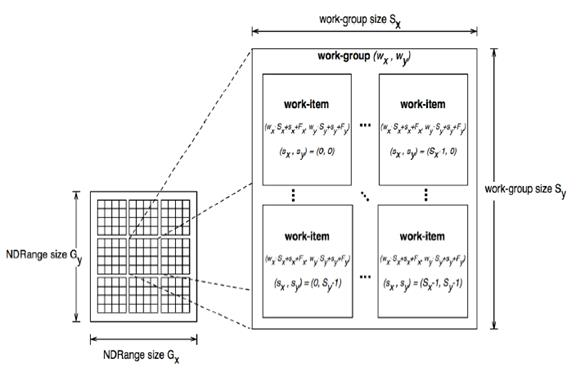
\includegraphics[width=0.8\textwidth]{index_space}
  \caption{Итерационное пространство в OpenCL. Источник: \cite{opencl3}}
  \label{fig:index_space}
\end{figure}

Низкоуровневый диалект вводит три новых типа данных: описание графа
(англ. \textit{Graph handle}), устройство (англ. \textit{device})
и событие (англ. \textit{event}). Описание графа -- указатель на специальную
структуру, которая содержит служебную информацию, например, список доступных
устройств. Устройство -- указатель на стуктуру, содержащую описание физического
устройства, на котором будет выполнено ядро. Событие -- указатель на структуру,
содержащую информацию о конкретном запуске ядра.

Результаты преобразования можно увидеть в листинге~\ref{lst:ath_rt_add} Приложения.

Дальнейшее понижение в LLVM IR подразумевает построение специальной структуры
данных, которая содержит в себе информацию об имени ядра, порядке и размерах
входных аргументов и итерационном пространстве. Именно она и передается
в библиотеку времени исполнения.

Полученный LLVM IR представлен в листинге~\ref{lst:llvm_add} Приложения.

Трансляция из одного диалекта в другой выполняется за счет стандартных средств
MLIR. Существует три вида конверсий:

\begin{enumerate}
  \item \textbf{Частичная} конверсия допускает, что некоторые операции исходного
  диалекта не могут быть преобразованы в целевой и будут оставлены без изменений.
  \item \textbf{Полная} конверсия требует преобразования всех операций. Если
  не удалось преобразовать хотя бы одну операцию, процедура считается неудачной.
  \item \textbf{Аналитическая} конверсия не выполняет реальных преобразований
  и лишь служит для получения отчета о том, какие операции исходного диалекта
  могут быть преобразованы в целевой.
\end{enumerate}
При этом разделяют три категории целевых операций:
\begin{enumerate}
  \item \textbf{Легальные.} Эти операции могут присутствовать в промежуточном
  представлении после завершения трансляции.
  \item \textbf{Динамически легальные.} При определении допусимости операции
  учитываются ее аргументы.
  \item \textbf{Нелегальные.} Эти операции не могут присутствовать ни в каком
  виде.
\end{enumerate}

Преобразование высокоуровневого диалекта в низкоуровневый использует схему
частичной конверсии, а преобразование низкоуровневого в LLVM IR -- полной.

Замена операций происходит с помощью шаблонов. Если находится операция,
соответствующая заранее заданному шаблону, то к ней применяется сопоставленный
ей алгоритм трансляции. При этом есть два ограничения:
\begin{enumerate}
  \item Исходная операция должна быть удалена или заменена набором других
  операций. Нельзя оставить операцию без изменений или изменить лишь ее аргументы.
  \item Решение о соответсвии операции шаблону может приниматься лишь на основании
  текущей операции. Другие операции (включая те, которыми были пораждены
  аргументы текущей операции) не могут принимать участия в этом процессе.
\end{enumerate}

\subsection{Библиотека времени исполнения}
Как показано на схеме~\ref{fig:compiler_scheme}, полученный LLVM IR передается
в JIT-компилятор. В качестве такого компилятора выступает рассмотренный ранее
ORC JIT. Итоговый бинарный файл сохраняется в оперативной памяти. В момент,
когда пользователь запрашивает вычисление графа, библиотека среды исполнения
обращается к JIT-компилятору, который возвращает ей указатель на функцию,
запускающую процесс исполнения.

Скомпилированный модуль так же может обращаться к библиотеке, чтобы загрузить
данные в память или запустить выполнение ядра на устройстве.

Ядра также предоставляются библиотекой. В качестве исходного языка для описания
ядер был выбран OpenCL C, а для их запуска стандарт OpenCL 3.0. Главная причина
-- открытость и переносимость стандарта (рис.~\ref{fig:api_layering}).

\begin{figure}[h]
  \centering
  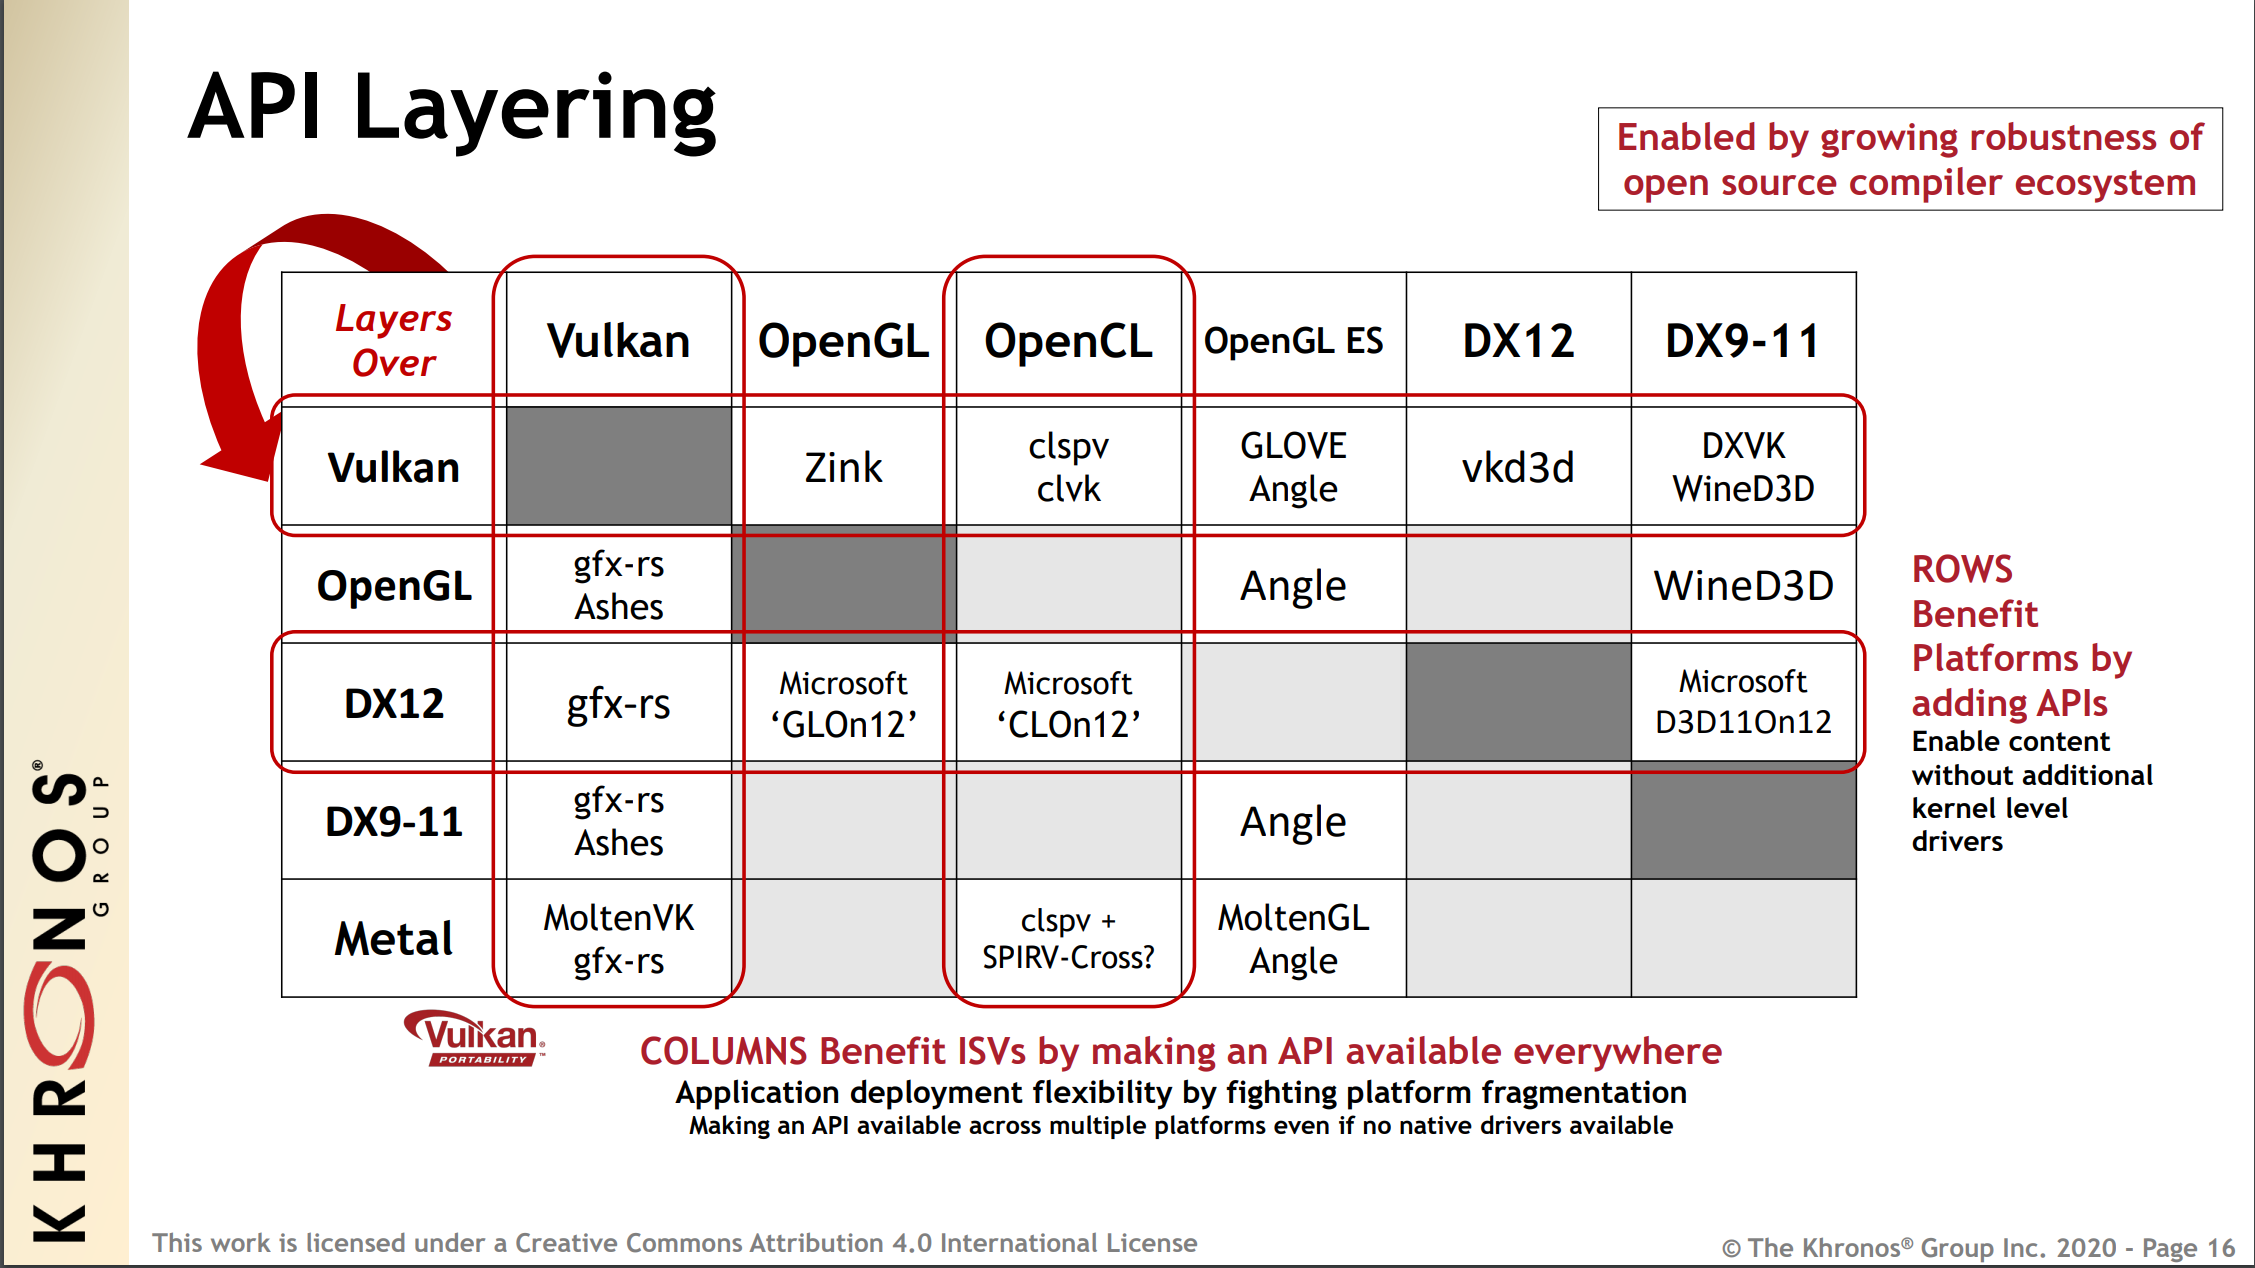
\includegraphics[width=\textwidth]{api_layering}
  \caption{Инструменты эмуляции различных стандартов. Источник: \url{https://www.khronos.org/assets/uploads/apis/OpenCL-3.0-Launch-Apr20.pdf}}
  \label{fig:api_layering}
\end{figure}

\subsubsection{Управление памятью}

Важная функция библиотеки -- управление памятью. Во время исполнения от бинарного
модуля могут поступать запросы на доступ к данным тензоров. Для этого необходимо
отыскать наиболее свежую копию данных, отправить ее на нужное устройство и
пометить этот тензор особым образом, чтобы предотвратить одновременный доступ
с нескольких устройств. Общая схема взаимодействия показана на 
рис.~\ref{fig:memory_management}.

\begin{figure}[h]
  \centering
  
\includegraphics[width=\textwidth]{memory_management}
  \caption{Схема взаимодействия исполняемого модуля и подсистемы управления памятью}
  \label{fig:memory_management}
\end{figure}

Перед запуском все устройства регистрируются в аллокаторе. При этом устройства
могут иметь собственные аллокаторы, а могут переиспользовать системный. Первый
случай возникает, когда у устройства есть собственная модель памяти, не
включающая в себя ОЗУ, например, при исполнении кода на выделенном GPU. Второй --
когда память устройства и ОЗУ -- одно и то же устройство, например, при
исполнении кода на CPU.

При поступлении запроса на выделение памяти под тензор создается специальная
запись, в которой отмечается виртуальный адрес тензора, размер выделяемого
участка памяти, метка версии и устройство, на котором находится эта запись.
Когда поступает запрос на запись в тензор, аллокатор убеждается, что к этой
области памяти больше никто не обращается, находит самую свежую версию записи
и копирует данные на нужное устройство. Если на устройстве закончилось свободное
пространство, аллокатор устройства может выгрузить часть ненужных данных в ОЗУ.
Если и на ОЗУ недостаточно памяти, то часть данных будет выгружена на диск.
Когда поступает уведомление об окончании работы с тензором, запись помечается
как доступная к использованию, но не удаляется с устройства. Это позволяет
избежать лишних копирований данных в случае, если повторный доступ будет
осуществлен на том же устройстве. Аналогичным образом обрабатываются запросы
на чтение тензоров. При этом нескольким устройствам одновременно разрешается
читать один и тот же тензор.
